\documentclass{beamer}

%Paquetes a usar
\usepackage{hyperref}
\usepackage{listings}
\usepackage{graphicx}

%Configuración del tema
\usetheme{Madrid}
\usecolortheme{whale}

%Estilo de código
\lstdefinestyle{micpp}{
	title=\lstname,
	language=C++,
	basicstyle=\tiny\ttfamily,
	breaklines=true, 
	keywordstyle=\color{blue},
	commentstyle=\color[rgb]{0,0.6,0},
  	identifierstyle=\color{orange},
 	stringstyle=\color{purple},
	tabsize=1,	
	escapechar=@,
}

\lstdefinestyle{miglsl}{
	title=\lstname,
	language=C++,
	basicstyle=\tiny\ttfamily,
	breaklines=true, 
	keywordstyle=\color{blue},
	commentstyle=\color[rgb]{0,0.6,0},
  	identifierstyle=\color{orange},
 	stringstyle=\color{purple},
	tabsize=1,	
	escapechar=@,
	morekeywords={
		vec2, vec3, vec4,
		mat2, mat3, mat4,
		uniform, sampler2d, sampler2D
	}
}

%Directorio de gráficos
\graphicspath{ {../images/} }

%Metadata
\title{Zuazo}
\subtitle{Librería para manipular video en tiempo real}
\author[Oier Lauzirika Zarrabeitia]{Oier Lauzirika Zarrabeitia 
	\\{
		\small \href{mailto:oier.lauzirika.zarrabeitia@alumnos.upm.es}{oier.lauzirika.zarrabeitia@alumnos.upm.es}}
	}
	
\institute[]{Estudiante de Ingeniería de Sonido e Imagen en la ETSI de Sistemas de Telecomunicación, Universidad Politécnica de Madrid}
\date[FF del CUSL 13]{Fase final del CUSL 13, 10/05/2019} 

%Al cominezo de cada sección
\AtBeginSection[]
{
	\begin{frame}
		\frametitle{Contenidos}
  		\tableofcontents[currentsection]
	\end{frame}
}

%Comenzamos con la presentación
\begin{document}

%
%Página del título
%

\begin{frame}
	\maketitle
	\begin{columns}
		\column{0.5\textwidth} 
\includegraphics[width=\textwidth]{zuazo_logo}
		\column{0.5\textwidth} 
\includegraphics[width=\textwidth]{cusl13_logo}
	\end{columns}
\end{frame}

%
% Sección de Introducción
%
\section{Introducción}

%¿Qué es Zuazo?
\begin{frame} \frametitle{¿Qué es Zuazo?}
	\begin{itemize}
		\item{Una librería para manipular video en tiempo real}
		\item{Escrita en C++17, incluyendo la API}
		\item{Soporta distribuciones GNU/Linux basadas en Debian} 
		\item{Emplea aceleración por GPU en la medida de lo posible}
	\end{itemize}
\end{frame}

%Librerias
\begin{frame} \frametitle{Librerías de terceros}
	\begin{itemize}
		\item{Librería estándar de C++}
		\item{OpenGL ES 3.0}
		\item{GLFW3 (a reemplazar por SDL2)}
		\item{FFmpeg}
		\item{Magick++}
		\item{nanoSVG (a reemplazar por rsvg)}
		\item{V4L2}
	\end{itemize}
\end{frame}

%Dinámica
\begin{frame} \frametitle{Dináminca}
	%TODO
\end{frame}

%
% E/S disponible y "procesadores"
%
\section{E/S disponible y "procesadores"}

%Entradas de video disponibles
\begin{frame}[t] \frametitle{Entradas de video disponibles}
	\begin{itemize}
		\item{Archivos de video} \pause
		\item{Archivos de imágenes} \pause
		\item{Archivos SVG} \pause
		\item{Dispositivos compatible con V4L2}
	\end{itemize}
\end{frame}

%Salidas de video disponibles
\begin{frame}[t] \frametitle{Salidas de video disponibles}
	\begin{itemize}
		\item{Ventana}
		\item{Monitor}
	\end{itemize}
\end{frame}

%Efectos basados en shaders de fragmento
\begin{frame}[t] \frametitle{Efectos basados en shaders de fragmento}
	\begin{itemize}
		\item{Corrección de tono, saturación y luminosidad (HSL)} \pause
		\item{Corrección de brillo y contraste} \pause
		\item{Color a escala de grises} \pause
		\item{Representación en luminancia del canal alpha}  \pause
		\item{Invertir color} \pause
		\item{A definir por el usuario}
	\end{itemize}
\end{frame}

%
% Documentación
%
\section{Documentación}

%Documentación
\begin{frame}[allowframebreaks] \frametitle{Documentación}
	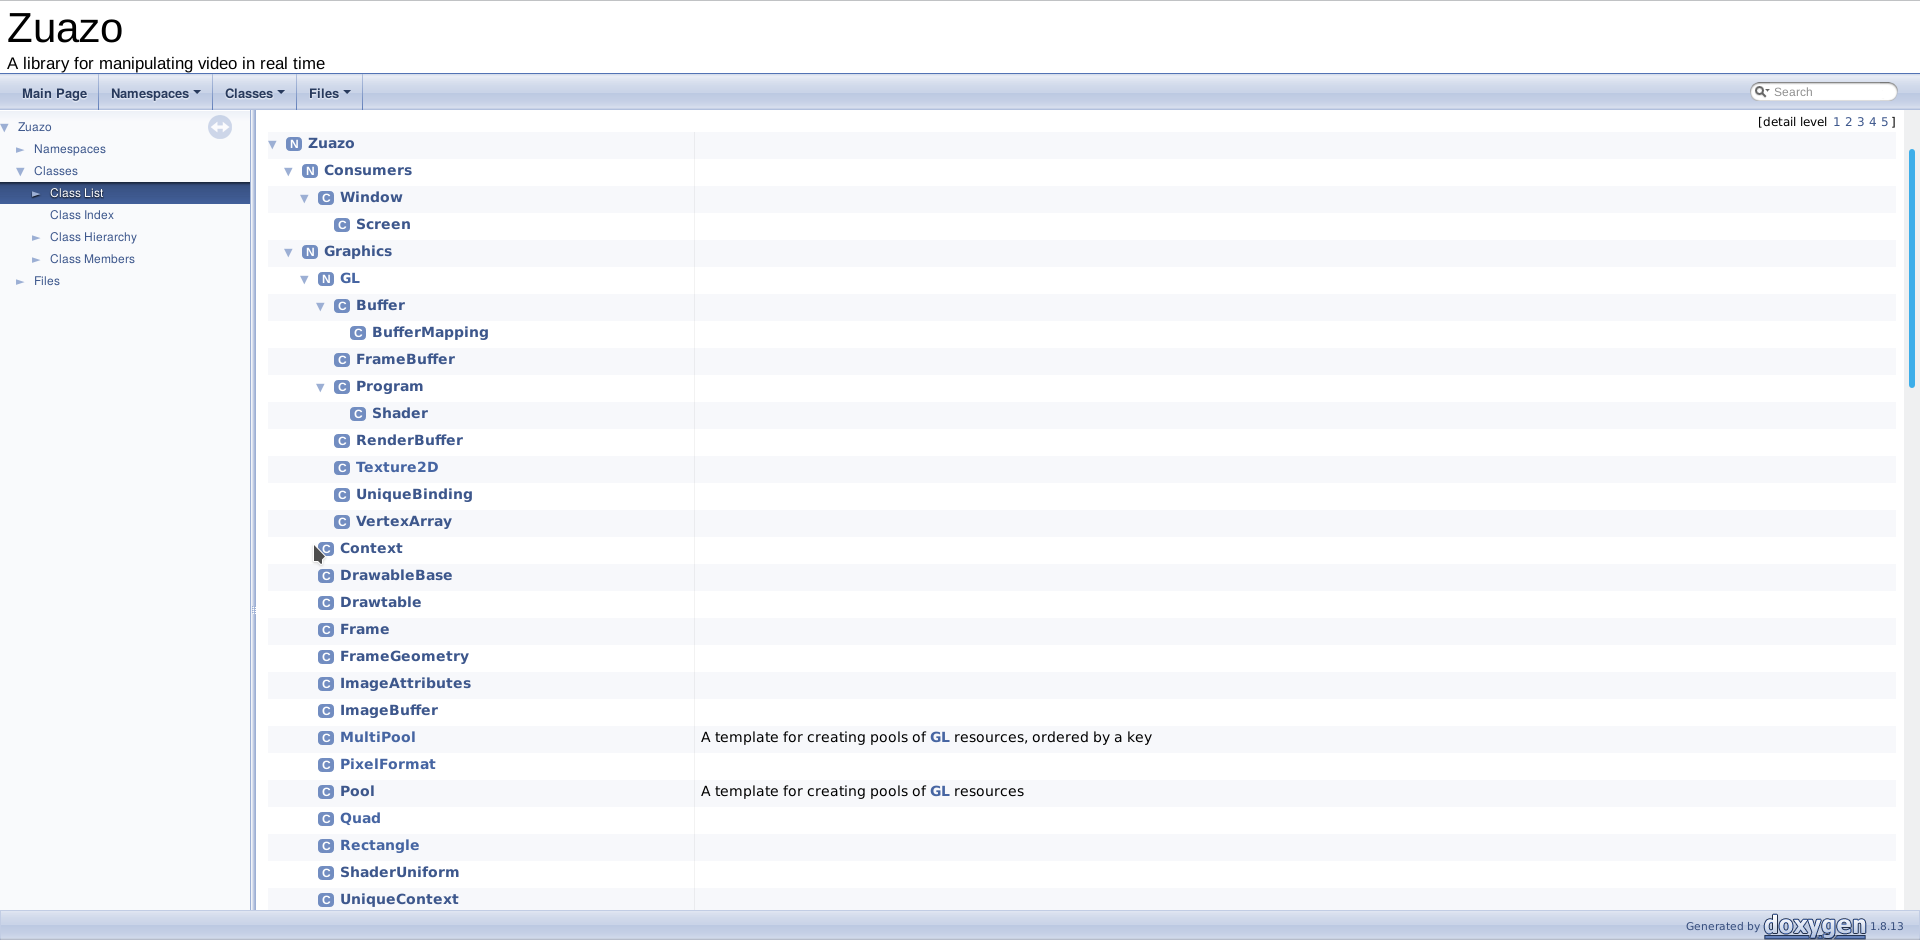
\includegraphics[width=\textwidth]{doxy1} 
	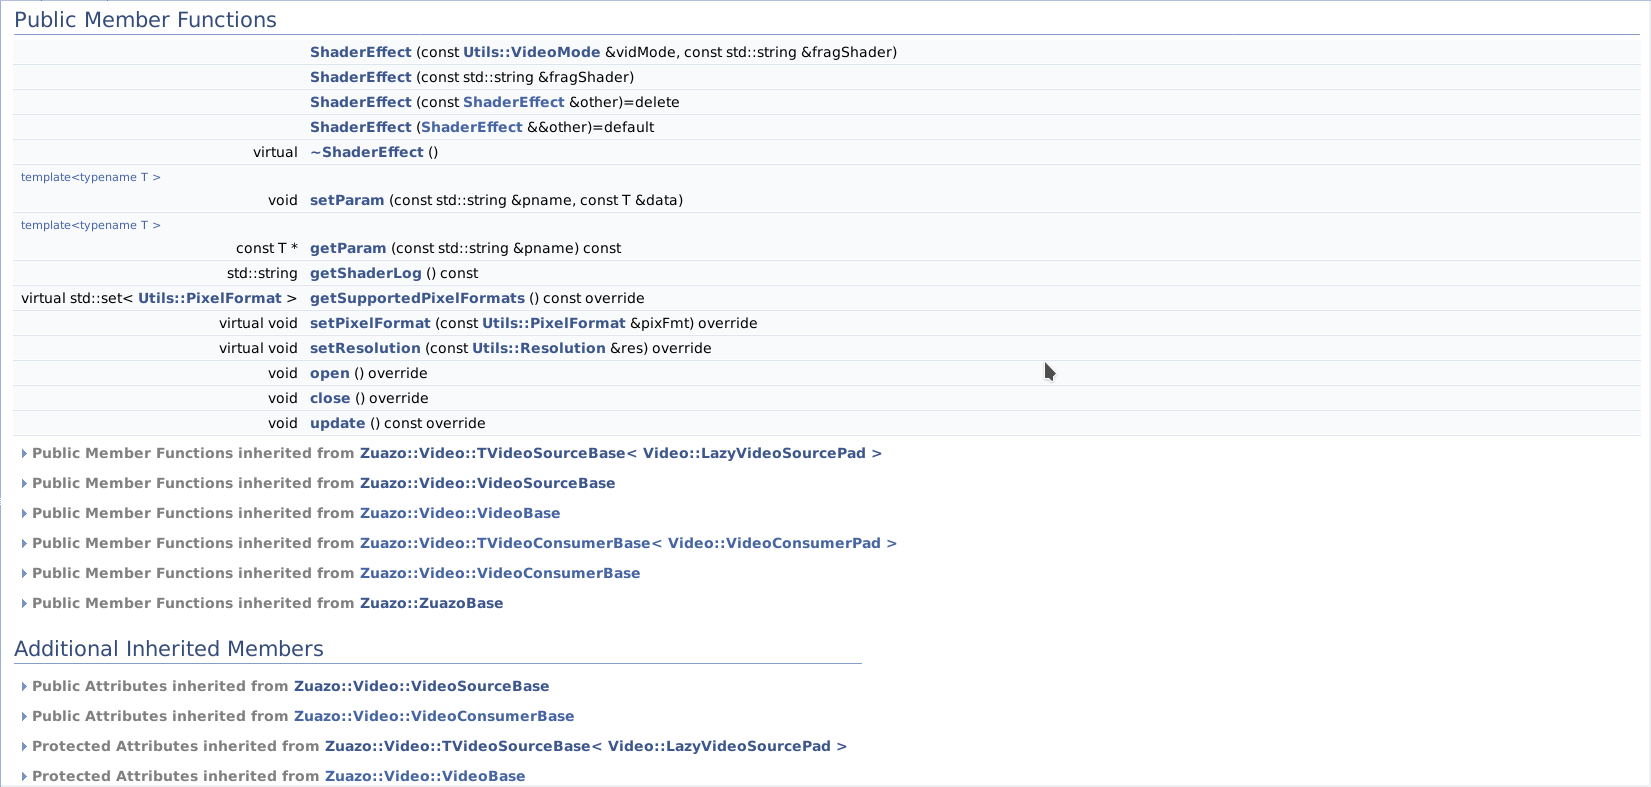
\includegraphics[width=\textwidth]{doxy2}
\end{frame}

%
% Ejemplos
%
\section{Ejemplos}

%¡Hola  Mundo!
\begin{frame}[t, allowframebreaks] \frametitle{Programa "¡Hola Mundo!"}
	\lstinputlisting[style=micpp]{../code/HolaMundo.cpp}
\end{frame}

%Creación de shaders de fragmento
\begin{frame}[t, allowframebreaks] \frametitle{Creación de shaders de fragmento}
	\lstinputlisting[style=miglsl]{../code/quantize.glsl}
	\lstinputlisting[style=micpp]{../code/Cuantizar.h}
	\lstinputlisting[style=micpp]{../code/Cuantizar.cpp}
	\lstinputlisting[style=micpp]{../code/CuantizarApp.cpp}	
\end{frame}


%
% Conclusiones
%
\section{Conclusiones}

%Estado del arte
\begin{frame} \frametitle{Estado del arte}
	%TODO
\end{frame}

%Cosas por hacer
\begin{frame} \frametitle{Cosas por hacer}
	%TODO
\end{frame}

%Bugs
\begin{frame} \frametitle{Bugs}
	\begin{itemize}
		\item{Transparencia independiente del orden (OIT) en el compositor}
		\item{Renderizado de color a formato de pixeles del tipo "Escala de grises" hace incorrectamente la conversión de luminancia}
	\end{itemize}
\end{frame}

%Agradecimientos
\begin{frame} \frametitle{Agradecimientos}
	\begin{itemize}
		\item{Blog \href{http://blogs.upm.es/softwarelibre/}{"Software libre en UPM"} mantenida por Laura Arjona Reina}
		\item{Hackelarre}
		\item{Organización del CUSL}
		\item{Mis padres, familia y amigos}
	\end{itemize}
\end{frame}

%Termina el ducumento
\end{document}
